\section{Results}
To analyze the effectiveness of our proposed methodology and visual system, we conducted three case studies. In this section we present the results of these three case studies. These case studies analyze three events that represent three types of abnormalities from the taxi data - increase in drop offs in a zone, decrease in drop offs in a zone, and a combination of both in two different zones.

\textbf{Case Study 1 - Halloween Week: } We first looked at the taxi-trends for the week of Halloween, and noticed an abnormal spike in the Civic center taxi zone (TriBeCa area) as seen in (Fig.~\ref{fig:tribecatrend}). To understand the potential motivation behind this, we looked at the topics and sentiment of the tweets from this taxi zone. There were significant proportion of tweets talking about Halloween (Celebration + Halloween topics) with almost all having a positive sentiment. We also noticed that people from the TriBeCa area tweeted ~6\% (14\% to 20\%) more during Halloween than during normal days. This indicated that there were many Halloween events happening in this zone that attracted people from different regions to the TriBeCa area. Further analysis can be done to understand the origin of people traveling to this zone for more observations.

\begin{figure}[h]
 \centering % avoid the use of \begin{center}...\end{center} and use \centering instead (more compact)
 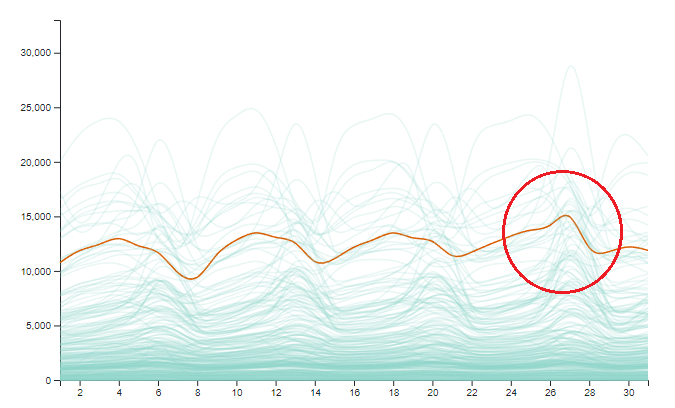
\includegraphics[width=\linewidth]{final/fig/Tribeca_taxi_trend.png}
 \caption{Trend of taxi drop offs by day in the TriBeCa zone}
 \label{fig:tribecatrend}
\end{figure}

Upon secondary research, it was understood that the TriBeCa area is widely popular for its Halloween events \cite{tribecanews} ranging from the long running tradition of Halloween Parade at the Washington Market Park to the events organized at the BMMC Tribeca Performing Arts Center which reinforced our hypothesis.


\textbf{Case Study 2 - Macy's Thanksgiving Parade: } This time, we noticed some decline in the number of drop-offs in the Logan Square East and Garment District zones during the Thanksgiving week. One of the major events that happens during this week is the Macy's parade. And it is typical for streets along the route of the parade to be closed down during this time and these two zones happen to be a part of the parade route. We also noticed that the ratio of tweets talking about the parade to the overall tweets from that region during the week was the highest for these two zones (~20\% tweets talking about the parade).

\begin{figure}[h]
 \centering % avoid the use of \begin{center}...\end{center} and use \centering instead (more compact)
 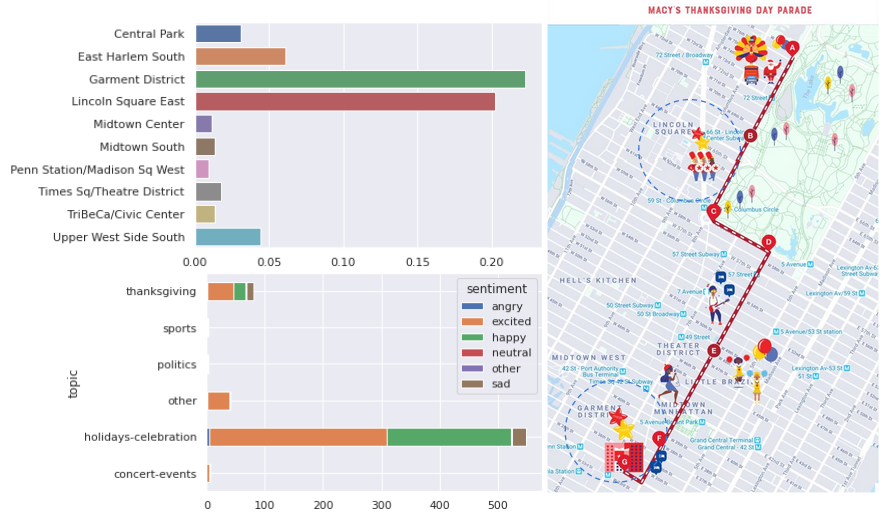
\includegraphics[width=\linewidth]{final/fig/Macys parade.png}
 \caption{Macy's parade route (right) and ratio of tweets talking about the parade by zone (top left)}
 \label{fig:macys}
\end{figure}

\textbf{Case Study 3 - Dec 31\textsuperscript{st} Celebration at Times Square: } For the final case study, we looked into the week of December 31\textsuperscript{st}. Here, from the Taxi data we noticed some abnormal increases in drop offs in the Clinton East zone and a sharp decline in drop offs in the Time Square zone. It is evident that the decline in the Time Square zone is due to the New Years celebration; the iconic Times Square ball drop event is widely famous around the world. Due to the event, the streets are typically closed off at the times square area. So naturally people look for a closer access point near Times Square, and Clinton East zone turns out to be one of those access points with streets offering entry into the Times Square area. Also, when we looked into the twitter data, we found a lot of conversations surrounding the traffic congestion as well.

These case studies confirm the effectiveness of the proposed framework of utilizing Taxi and Twitter data to understand urban movements and social behavior to some extent and raise other questions that can be explored further.
